% The four tiers of a value hierarchy.
%
%   figures/tikz/ds-value-hierarchy.tex
%       -> media/figures/ds-value-hierarchy.{png,svg}
%
% Lecture 11 (Optimization for Decision Support), section III, Definition 11.1.
% Source: Driscoll, Parnell & Henderson (eds., 2023), Decision Making in Systems
% Engineering and Management, 3rd ed., S6.2, printed p. 230: "A value hierarchy
% consists of four tiers: a project fundamental objective, major functions and
% subfunctions, performance objectives, and value measures." Each performance
% objective is paired with one value measure (the scale a candidate is scored on).
% The branching (2 functions, 3 objectives) is generic, not an example from the book.
%
% GREYSCALE: black and grey only; the tier names are printed text, so nothing is
% carried by colour.
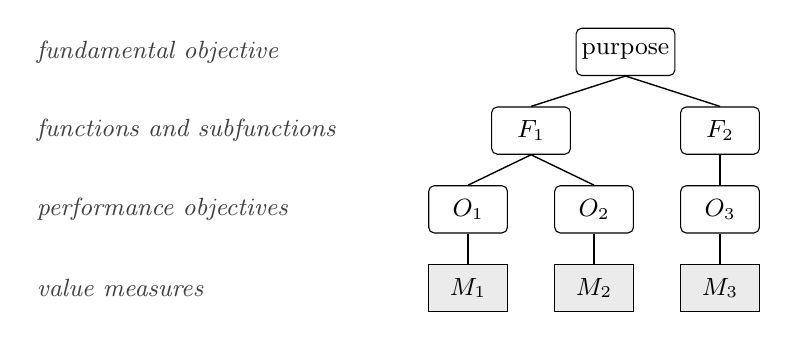
\begin{tikzpicture}[
    font=\small,
    node/.style={draw=black, fill=white, rounded corners=2pt, minimum width=10mm,
                 minimum height=6mm, inner sep=2pt},
    measure/.style={node, sharp corners, fill=black!8},
    tier/.style={font=\small\itshape, anchor=west, text=black!75},
    link/.style={draw=black, line width=0.5pt},
  ]
  % tier labels (left column)
  \node[tier] at (0,3.0) {fundamental objective};
  \node[tier] at (0,2.0) {functions and subfunctions};
  \node[tier] at (0,1.0) {performance objectives};
  \node[tier] at (0,0.0) {value measures};
  % tree
  \node[node] (P)  at (7.6,3.0) {purpose};
  \node[node] (F1) at (6.4,2.0) {$F_1$};
  \node[node] (F2) at (8.8,2.0) {$F_2$};
  \node[node] (O1) at (5.6,1.0) {$O_1$};
  \node[node] (O2) at (7.2,1.0) {$O_2$};
  \node[node] (O3) at (8.8,1.0) {$O_3$};
  \node[measure] (M1) at (5.6,0.0) {$M_1$};
  \node[measure] (M2) at (7.2,0.0) {$M_2$};
  \node[measure] (M3) at (8.8,0.0) {$M_3$};
  \draw[link] (P.south) -- (F1.north);
  \draw[link] (P.south) -- (F2.north);
  \draw[link] (F1.south) -- (O1.north);
  \draw[link] (F1.south) -- (O2.north);
  \draw[link] (F2.south) -- (O3.north);
  \draw[link] (O1) -- (M1);
  \draw[link] (O2) -- (M2);
  \draw[link] (O3) -- (M3);
\end{tikzpicture}
